\documentclass[aspectratio=169,xcolor={dvipsnames,table}]{beamer}
\usepackage[no-math,deluxe,expert,haranoaji]{luatexja-preset}
\usepackage{luatexja-otf}
\renewcommand{\kanjifamilydefault}{\gtdefault}
\renewcommand{\emph}[1]{{\upshape\bfseries #1}}
\usetheme{metropolis}
\metroset{block=fill}
\setbeamertemplate{navigation symbols}{}
\usecolortheme[rgb={0.7,0.2,0.2}]{structure}
%%%%%%%%%%%%%%%%%%%%%%%%%%%
\usepackage{media9}
%%%%%%%%%%%%%%%%%%%%%%%%%%%
%% さまざまなアイコン
%%%%%%%%%%%%%%%%%%%%%%%%%%%
\usepackage{fontawesome}
\usepackage{figchild}
\usepackage{twemojis}
\usepackage{utfsym}
\usepackage{bclogo}
\usepackage{marvosym}
\usepackage{fontmfizz}
\usepackage{pifont}
\usepackage{phaistos}
\usepackage{worldflags}
\usepackage{jigsaw}
%%%%%%%%%%%%%%%%%%%%%%%%%%%
\usepackage{tikz}
\usetikzlibrary{backgrounds}
\usepackage{tcolorbox}
\usepackage{tikzpeople}
\usepackage{circledsteps}
\usepackage{xcolor}
\usepackage{amsmath}
\usepackage{booktabs}
\usepackage{chronology}
\usepackage{signchart}
%%%%%%%%%%%%%%%%%%%%%%%%%%%
%% 場合分け
\usepackage{cases}
%%%%%%%%%%%%%%%%%%%%%%%%%%%
% \myAnch{<名前>}{<色>}{<テキスト>}
% 指定のテキストを指定の色の四角枠で囲み, 指定の名前をもつTikZの
% ノードとして出力する. 図には remeber picture 属性を付けている
% ので外部から参照可能である.
\newcommand*{\myAnch}[3]{%
  \tikz[remember picture,baseline=(#1.base)]
    \node[draw,rectangle,#2] (#1) {\normalcolor #3};
}
%%%%%%%%%%%%%%%%%%%%%%%%%%%%
%% 音声リンク表示
\newcommand{\myaudio}[1]{\href{#1}{\faVolumeUp}}
%%%%%%%%%%%%%%%%%%%%%%%%%%%
% \myEmph コマンドの定義
%\newcommand{\myEmph}[3]{%
%    \textbf<#1>{\color<#1>{#2}{#3}}%
%}
\usepackage{xparse} % xparseパッケージの読み込み
\NewDocumentCommand{\myEmph}{O{} m m}{%
    \def\argOne{#1}%
    \ifx\argOne\empty
        \textbf{\color{#2}{#3}}% オプション引数が省略された場合
    \else
        \textbf<#1>{\color<#1>{#2}{#3}}% オプション引数が指定された場合
    \fi
}
%%%%%%%%%%%%%%%%%%%%%%%%%%%
%% 文末の上昇イントネーション記号 \myRisingPitch
%% 通常のイントネーション \myDownwardPitch
%% https://note.com/dan_oyama/n/n8be58e8797b2
%%%%%%%%%%%%%%%%%%%%%%%%%%%
\newcommand{\myRisingPitch}{
\begin{tikzpicture}[scale=0.3,baseline=0.3]
\draw[->,>=stealth] (0,0) to[bend right=45] (1,1);
\end{tikzpicture}
}
\newcommand{\myDownwardPitch}{
\begin{tikzpicture}[scale=0.3,baseline=0.3]
\draw[->,>=stealth] (0,1) to[bend left=45] (1,0);
\end{tikzpicture}
}
%%%%%%%%%%%%%%%%%%%%%%%%%%%
\title{English is fun.\,\,{}--- I have watched the movie three times. ---}
  \author{}
\institute[]{}
\date[]

%%%%%%%%%%%%%%%%%%%%%%%%%%%%
%% TEXT
%%%%%%%%%%%%%%%%%%%%%%%%%%%%
\begin{document}
\begin{frame}[plain]
  \titlepage
\end{frame}

\section*{授業の流れ}
\begin{frame}[plain]
  \frametitle{授業の流れ}
  \tableofcontents
\end{frame}

\section{現在完了--経験--}
\subsection{現在完了とは(復習)}

\begin{frame}<1-3>[plain]{現在完了とは(復習)}
 \begin{enumerate}
 \item Jane has stayed in London for six years.\visible<2->{\small (継続)}
 \item I have watched the movie three times.\visible<3->{\small (経験)}
 \item Bob has lost his bag.
\end{enumerate}



 \begin{exampleblock}{Topic for Today}
\small
\begin{itemize}
 \item  $\text{現在完了(}=\textcolor{NavyBlue}{\text{have} + \text{過去分詞\,)}}$%
は「過去と現在にまたがる表現」です
\item 主語が三人称単数のときは {\textcolor{NavyBlue}{\bfseries has $+$ 過去分詞}}
\end{itemize}
      \end{exampleblock}
\end{frame}

\subsection{現在完了--経験--}
\begin{frame}[plain]{現在完了--経験--}
 
\visible<1->{\begin{enumerate}%\setcounter{enumi}{1}
 \item $\left\{\begin{tabular}{rl}
(A)& I \textcolor{Maroon}{\bfseries visited} the tower two years ago.\hspace{9\zw}{\small tower: 塔、タワー}\\
(B)& I \textcolor{NavyBlue}{\bfseries have visited} the tower three times.
\end{tabular}
\right.$
\end{enumerate}}

\visible<2->{\signchart[width=10,height=.5]{,,,,,{\textcolor{Maroon}{visited}},,今}{,,},}
\visible<3->{\signchart[width=10,height=.5]{1回目,,2回目,,{\textcolor{NavyBlue}{have visited}},,3回目,}{,,,}}

\begin{tikzpicture}[overlay]
%\draw[gray!50] (0,0) grid (12,5);
 %\fill[ForestGreen!70,opacity=.5] (11.57,3.75) circle [radius=.25];
\visible<2->{ \fill[Maroon!90,opacity=.75] (8.675,3.8) circle [radius=.25];}
\visible<3->{\fill[NavyBlue!90,opacity=.75] (3.1,1.21) circle [radius=.25];
\fill[NavyBlue!90,opacity=.75] (5.35,1.21) circle [radius=.25];
\fill[NavyBlue!90,opacity=.75] (9.78,1.21) circle [radius=.25];}
%\node[fill=NavyBlue!90,opacity=.75] at (10.88,1.21) { };
\visible<4->{\node[] at (10.89,1.21) {\LARGE \textcolor{NavyBlue}{x }};
\node[] at (10.9,.4) {\scriptsize \begin{tabular}{c}
				   これまでに\\
				 3回訪れた\\
				  ことがある\end{tabular}};}
% \draw[NavyBlue!70,line width=6pt,opacity=.7] (4.2,1.21) -- (10.9,1.21);
\end{tikzpicture}

\visible<5->{過去から現在までの「経験」を表しています}
\end{frame}

\subsection{頻度を表す表現}
\begin{frame}[plain]{頻度を表す表現}


 \begin{enumerate}
  \item \visible<1->{I have met the singer once.\hfill{\small met: meetの過去分詞}}\\
\visible<2->{\small わたしはその歌手に一度あったことがある。}
  \item  \visible<1->{My mother has visited Taiwan twice.\hfill{\small visit: 訪れる}}\\
\visible<3->{\small 母は台湾を二度訪れたことがある。}
  \item \visible<1->{He has seen the movie three times.\hfill{\small seen: seeの過去分詞}\\}
\visible<4->{\small 彼はその映画を三回見たことがある。}
  \item \visible<1->{They have traveled to Paris many times.\hfill{\small travel:旅行する}}\\
\visible<5->{\small 彼らはパリに何度も旅行したことがある。}
\end{enumerate}

\begin{exampleblock}<6->{「何回」という表現}
\small

{\rowcolors{2}{NavyBlue!50}{yellow!50}
\begin{tabular}{ll}
意味&英語\\
1回 &once \\
2回 &twice \\
3回& three times\\
\end{tabular}}
{\rowcolors{2}{NavyBlue!50}{yellow!50}
\begin{tabular}{ll}
&\\
4回&four times\\
5回&five times \\
6回&six times \\
\end{tabular}}
{\rowcolors{2}{NavyBlue!50}{yellow!50}
\begin{tabular}{ll}
&\\
7回&seven times\\
8回&eight times \\
9回&nine times \\
\end{tabular}}
{\rowcolors{2}{NavyBlue!50}{yellow!50}
\begin{tabular}{ll}
&\makebox[0pt][r]{文の最後におきます}\\
10回&ten times\\
\multicolumn{1}{c}{$\vdots$}&\multicolumn{1}{c}{$\vdots$} \\
何回も&many times \\
\end{tabular}}
      \end{exampleblock}



\end{frame}


\begin{frame}[plain]{否定と疑問文}
\Large

 \begin{enumerate}
  \item \visible<1->{I have \textcolor{Maroon}{\bfseries never} eaten sushi.}\hfill{}\visible<2->{{\small eaten: eatの過去分詞}}
  \item \visible<3->{Have you \textcolor{ForestGreen}{\bfseries ever} climbed a mountain?}\hfill{}\visible<4->{{\small climb: 登る}}
 \end{enumerate}

\vfill

\begin{exampleblock}<5->{Topics for Today}
\small
\begin{itemize}
 \item \visible<6->{neverは「今までに一度もない」という否定の意味(置き場所はnotと同じ)}
 \item \visible<7->{everは疑問文で用いて「今までに」という意味}\\
\visible<8->{ Have you  ever $+$ 過去分詞 \ldots ?{{\footnotesize (あなたは今までに〜したことがありますか)}}}
\end{itemize}
\end{exampleblock}
\end{frame}


\begin{frame}[plain]{Exercises}
あたえられた日本語の意味になるよう(~~~~~~~~)内の語句を並べ替えましょう。なお、先頭の語は大文字で初めてください。

\vspace{-10pt}
 \begin{enumerate}
  \item あなたは今までにギターを弾いたことがありますか?\scalebox{3}{\twemoji{guitar}}\\
( you / have / ever / played ) the guitar?\\
\visible<2->{Have you ever played the guitar?}
\vspace{-10pt}
  \item あなたは今までにメキシコ料理を食べたことがありますか?\hfill\raisebox{-5pt}{\scalebox{3}{\twemoji{1f32e}}}\,\scalebox{.4}{\worldflag{MX}}\,\scalebox{3}{\twemoji{desert}}\\
( you / have / eaten / ever ) Mexican food?\\
\visible<3->{Have you ever eaten Mexican food?}
  \item 私は一度もジグソーパズルを買ったことがありません。\\
( never / have / I / bought ) a jigsaw puzzle.\\
\visible<4->{I have never bought a jigsaw puzzle.}
%  \item 私は一度も山に登ったことがない。
%(  climbed / I / never /  have ) a mountain.\\
%\visible<5->{I have never climbed a mountain.}
 \end{enumerate}

\vspace{-65pt}

\mbox{}\hfill\scalebox{.5}{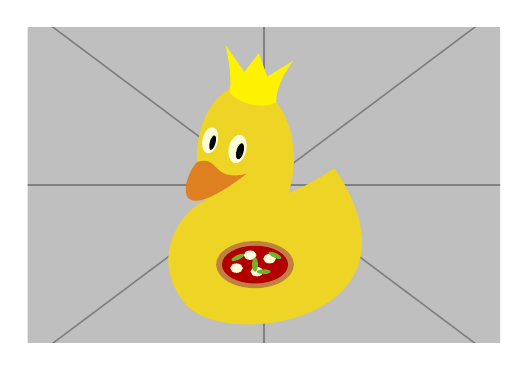
\begin{tikzpicture}
\clip (0,0) rectangle (6,4);
\node at (3,2) {%
\includegraphics[
width=8cm,height=6cm
]{example-image-duck}%
};
\jigsaw{6}{4}
\end{tikzpicture}}
\end{frame}

\end{document}
  \item  Have you ever eaten Mexican food?
